\documentclass[12pt,a4paper]{ctexart}
\usepackage[final]{pdfpages}
\usepackage{fancyhdr}
\usepackage{lastpage}
\usepackage{xcolor}
\usepackage{cite}
\pagestyle{fancy}
\fancyhf{}
\fancyhead[L]{\textcolor[gray]{0.6}{\leftmark}}
\fancyhead[R]{\textcolor[gray]{0.6}{\rightmark}}
\fancyfoot[C]{\textcolor[gray]{0.6}{第\thepage 页~共\pageref{LastPage}页}}
\renewcommand{\headrulewidth}{0pt}
\renewcommand{\footrulewidth}{0pt}
\setCJKmainfont{SimSun}[AutoFakeBold,AutoFakeSlant]
\setmainfont{TeX Gyre Termes}
\linespread{1.5}
\ctexset {
section = {
name = {第,章},
number = \chinese{section},
},
subsection = {
name = {第,节},
number = \chinese{subsection},
}
}
\date{}




\title{\Huge\textbf{2023年全国大学生信息安全竞赛\\作品报告}}
\begin{document}
\maketitle
\vspace{6cm}
{
    \Large\textbf{作品名称}:\textbf{\underline{\makebox[10cm]{基于TrustZone-M函数级内存地址}}}

    \textbf{\underline{\makebox[13cm]{空间随机化的可信实时系统}}}

    \textbf{电子邮箱}:\underline{\makebox[10cm]{\textbf{213211377@seu.edu.cn}}}

    \textbf{提交时间}:\underline{\makebox[10cm]{\textbf{\today}}}
}
\thispagestyle{empty}
\clearpage
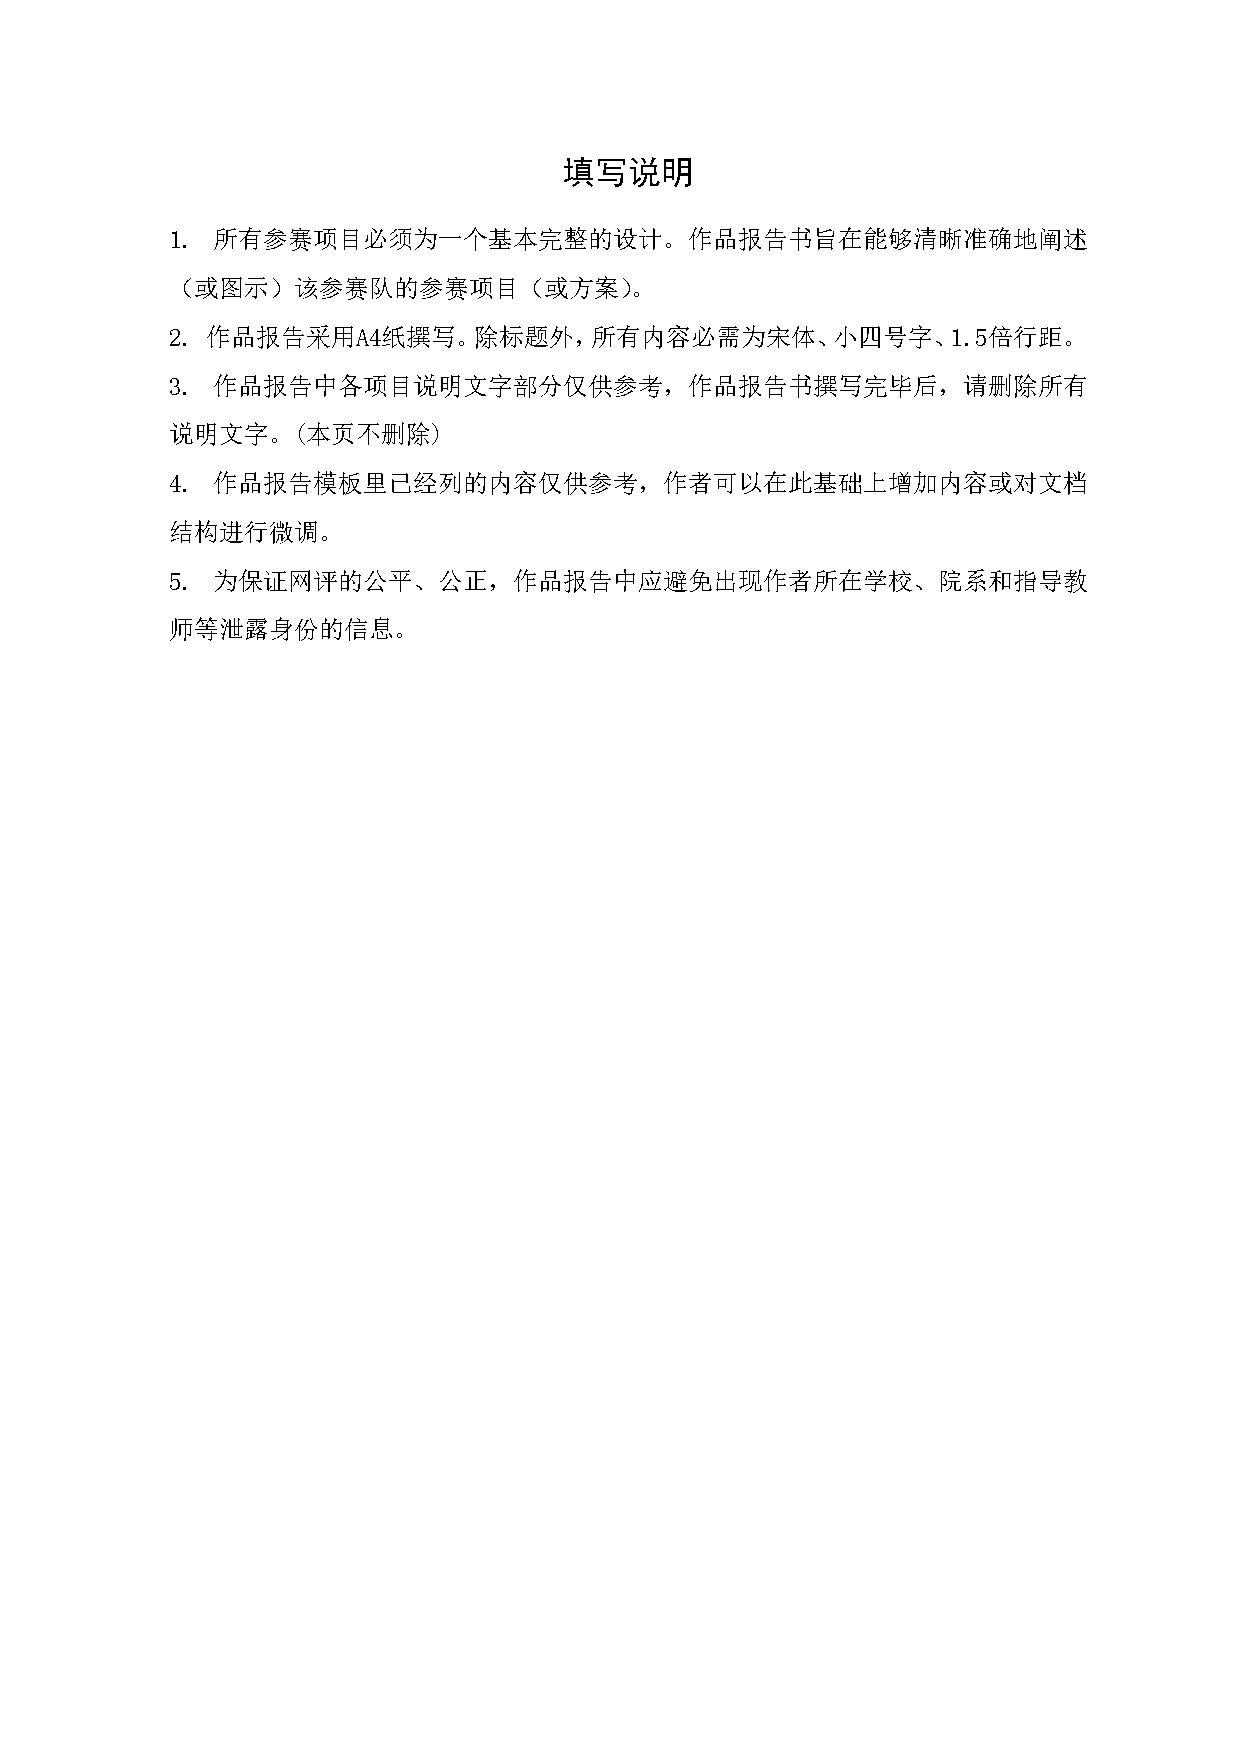
\includepdf{src/request.pdf}
\thispagestyle{empty}
\clearpage
\tableofcontents
\thispagestyle{empty}
\clearpage
\setcounter{page}{1}
\section*{摘要}
\addcontentsline{toc}{section}{摘要}
\thispagestyle{empty}
简要说明创作本作品之动机、功能、特性、创新处、实用性等.
\clearpage
\section{作品概述}
\subsection{作品背景}
可包括背景分析、研究现状、特色描述、应用前景分析等
\subsection{研究现状}
\par 随着ARMv8-M架构设备在物联网市场的逐渐普及,低端嵌入式系统的安全性近年来受到广泛关注。现有研究主要集中在以下几个关键领域,以解决低端嵌入式系统面临的安全挑战。首先,现有相关研究提出基于TrustZone-M技术的可信执行环境构建技术,其主要目的是为低端嵌入式设备提供可信软件服务,通过安全的通信机制使用户应用程序能够调用安全服务从而提高系统安全性。其次,面向低端嵌入式系统的OTA技术安全风险是一个重要领域,研究人员致力于解决OTA过程中可能面临的各种安全威胁。另外,Trusted firmware-M开源固件项目提供了一个综合性的安全框架,用于保护Arm Cortex-M设备的安全性。此外,面向低端嵌入式系统的内存破坏防御技术针对内存破坏攻击威胁进行研究,主要包括控制流完整性保护和地址空间信息隐藏技术。最后,ASLR(Address Space Layout Randomization)地址空间布局随机化技术提出了一种从另一个角度对系统进行保护的安全技术。这些研究领域的进展对于提高低端嵌入式系统的安全性具有重要意义。
\subsubsection{基于TrustZonc-M技术的可信执行环境构建技术}
一般来说,可信执行环境由可信执行环境操作系统(Trusted Execution EnvironmentOperating System,TEE OS)以及安全服务(或称为TA,Trusted Application)构成,可信执行环境操作系统主要为用户调用安全服务提供安全的通信机制。ARM TrustZone技术是ARM 公司2008年提出的处理器级系统范围的可信执行环境解决方案,为Cortex-A 系列芯片提供安全的可信执行环境支持。目前,大多数智能手机已配备有TrustZone的芯片以及可信执行环境操作系统,并安装了相应的安全服务以用于手机的安全支付、指纹服务、文件保密等。为了满足低端嵌入式系统对安全日益增长的需求,ARM在2015年提出了面向Cortex-M系列芯片的TrustZone-M8技术并支持ARMv8-M架构设备。基于TrustZone-M的低端嵌入式系统在物联网市场正逐渐普及,然而,面向资源受限设备的可信执行环境研究在学术界和工业界尚处于起步阶段。
(1)TrustZone-M 技术的安全机制
\par TrustZone-M面向资源受限的低端嵌入式设备,利用系统级的硬件隔离技术将系统资源分为安全/非安全世界。安全世界的资源可以访问非安全世界的资源,反之则会产生错误。下面从编程模型、资源分配以及异常处理三方面对TrustZone-M进行介绍。
\par 编程模型:自ARMv7-M架构开始,处理器有两种操作模式:thread模式和 handler模式。在thread模式下,处理器用于执行应用程序代码且其访问权限级别可以处于特权态(Privileged)或者非特权态(Unprivileged)。在 handler模式下,处理器用于执行异常处理程序代码且总是特权态。ARMv8-M架构引入TrustZone-M技术后,处理器额外增加了两个安全状态:安全态(Secure State)和非安全态(Non-secure State),这两个状态和处理器操作模式互相独立,即每个安全状态都有thread或者handler两个操作模式。安全状态不是由某一安全位控制,而是取决于处理器所访问的内存地址或者IO地址是映射在安全还是非安全世界。若该内存映射在安全世界,则处理器状态为安全态,反之,则为非安全态。不同的安全状态以及处理器操作模式对应不同的栈指针寄存器,共有PSP_NS、PSP_S、MSP_NS、MSP_S 四个栈指针寄存器,程序当前所使用的寄存器由当前处理器的状态决定,其中,thread 模式可以使用PSP (Process Stack Pointer>栈指针寄存器,也可以使用MSP (Main Stack Pointer)栈指针寄存器,而handler模式只能使用MSP栈指针寄存器。此外,支持 TrustZone-M 的ARMv8-M架构为两个安全状态分配了独立的CONTROL寄存器以及异常处理控制寄存器(PRIMASK、FAULTMASK、BASEPRI)。
\par 安全/非安全世界的切换通过三条新引入的指令实现:用于从非安全世界跳转至安全世界指令BXNS (Branch and Exchange Non-secure)、安全网关指令SG (SecureGateway)以及用于从安全世界链接跳转至非安全世界指令BLXNS (Branch with Linkand Exchange Non-secure)。安全世界程序调用非安全世界程序一般使用BLXNS 指令,然而,非安全世界程序不能直接调用安全世界程序,它必须首先跳转至该程序在一块特殊的安全世界内存区域的入口,该内存区域被称为非安全可调用(Non-SecureCallable,NSC)区域。为保证入口是从非安全世界至安全世界的有效跳转,入口的第一条指令必须为SG。当安全世界程序执行完成后,使用BXNS指令即可返回至非安全世界。此外,异常处理时也可以发生安全状态的切换。
\par 基于TrustZone-M设备的系统运行机制如图1-1所示,当设备上电启动之后,首先会执行安全世界的固件程序,包括安全启动(①)以及TrustZone-M的初始化(②),其中,TrustZone-M 的初始化主要涉及对资源的安全属性划分与配置。然后,由安全世界将控制权转交给非安全世界的启动代码(③)并进行非安全世界的初始化(④和)。在此之后,系统运行非安全世界的应用程序,在运行过程中,非安全世界可以通过调用安全世界的API以在安全世界执行相应任务,同样的,安全世界在执行过程中也可以通过回调函数调用非安全世界的函数。
\par 资源分配:TrustZone-M 技术为ARMv8-M架构设备提供基于硬件的内存隔离机制,处理器根据内存映射可以对所有资源(包括内存,外设等)进行访问,其内存资源可以设置不同的安全属性以及资源访问控制权限。内存资源可以通过安全属性单元(Security Attribution Unit,SAU)进行安全区域的划分,区域数量由芯片制造商决定,一般为8个区域,SAU只能在处理器处于安全状态下被配置。除SAU之外,安全属性还可以通过实现定义属性单元(Implementation Defined Attribution Unit,IDAU)来进行配置。对某一内存区域来说,其安全属性取决于SAU和IDAU对其配置的共同作用结果,通过对两种配置取逻辑或操作以确定最终的安全属性。此外,内存资源可以通过内存保护单元(Memory Protection Unit,MPU)进行内存访问权限的设置,包括读权限、写权限、可执行权限。任何未遵守该权限要求的访问将会触发HardFault 异常处理,安全/非安全世界各有一个MPU。
\section{作品设计与实现}
可包括系统架构设计、系统实现方案、系统实现功能等
\section{作品测试与分析}
可包括测试方案、测试环境搭建、测试数据及分析等
\section{创新性说明}
\section{总结}
\bibliographystyle{plain}
\bibliography{ref}
\end{document}